\documentclass[@BEAMER_OPTIONS@]{beamer}
    @USE_PGFPAGES@

    \usetheme[alternativetitlepage=true,titleline=true]{Torino}
    \setbeamertemplate{navigation symbols}{}
    \setbeamertemplate{note page}[plain]
    \setbeamertemplate{caption}{\insertcaption}

    \usepackage[utf8]{inputenc}
    \usepackage{graphicx}
    \usepackage{subfigure}
    \usepackage{xspace}
    \usepackage{adjustbox}
    \usepackage{tikz}
    \usepackage{relsize}
    \usepackage{fancyvrb}
    \fvset{fontsize=\footnotesize}
    \RecustomVerbatimEnvironment{verbatim}{Verbatim}{}
    \usepgflibrary{arrows}
    \usetikzlibrary{shadows,decorations.pathreplacing,patterns,shapes}
    \tikzstyle{every picture}=[semithick,>=stealth,remember picture]
    \usepackage{listings}
    \lstset{
        language=C++,
        basicstyle=\footnotesize,
        commentstyle=\color{chameleon1}\it\rmfamily,
        stringstyle=\color{chameleon4},
        numbers=left,
        numberstyle=\tiny,
        aboveskip=-0.02\baselineskip,
        belowskip=-0.02\baselineskip,
        columns=flexible,
        extendedchars=false,
        showstringspaces=false,
        morekeywords={global,kernel,ulong,size_t,get_global_id,get_global_size}
        }
    \newcommand{\code}[1]{\lstinline|#1|}
    \newcommand{\additive}{\hspace{1cm}\footnotesize(\emph{Additive expressions only})}
    \newcommand{\singledevice}{\hspace{1cm}\footnotesize(\emph{Single-device contexts})}
    \protected\def\plusplus{{\nolinebreak[4]\hspace{-.05em}\raisebox{.4ex}{\relsize{-3}\bf ++}}\xspace}
    \newcommand{\CXX}{{\rm C}\plusplus}
    \newcommand{\CC}{{\rm C99}\xspace}
    \usepackage{ifthen}
\usetikzlibrary{shadows.blur}
\newlength{\forkmeoffset}
\setlength{\forkmeoffset}{3em}

\newcommand{\forkme}[2]{
  \ifthenelse{\equal{#1}{east}}{%
    \tikzset{forkmerot/.style={rotate=-45}}
  }{%
    \tikzset{forkmerot/.style={rotate=45}}
  }
  \begin{tikzpicture}[remember picture, overlay]
    \node[forkmerot, shift={(0, -\forkmeoffset)}] at (current page.north #1) {
      \begin{tikzpicture}[remember picture, overlay,scale=0.5]
        \node[
            fill=chameleon1,
            text centered,
            minimum width=50em,
            minimum height=1.2em,
            blur shadow,
            shadow yshift=0pt,
            shadow xshift=0pt,
            shadow blur radius=.2em,
            shadow opacity=50,
            text=white
            ](fmogh) at (0pt, 0pt) {
                \fontfamily{phv}\selectfont\bfseries\tiny%
                \href{#2}{Fork me on GitHub}
            };
        \draw[
            white,
            dashed,
            line width=.04em,
            dash pattern=on .2em off 1.5\pgflinewidth
            ] (-25em,1em) rectangle (25em,-1em);
      \end{tikzpicture}
    };
  \end{tikzpicture}
}

    \tikzset{
        treenode/.style={
            draw,
            fill=white,
            blur shadow,
            shadow xshift=1pt,
            shadow yshift=-1pt,
            shadow blur radius=2pt,
            shadow opacity=40
            }
        }


    \title{VexCL}
    \subtitle{GPGPU Without the Agonizing Pain}

    \author{Denis Demidov}
    \institute{
        Supercomputer Center of Russian Academy of Sciences
        \\ \vspace{\baselineskip}
        }
    \date{
        \href{http://meetingcpp.com/index.php/schedule14.html}{CIMNE, Barcelona, 09.2015}
    }


\begin{document}

%----------------------------------------------------------------------------
\begin{frame}{}
    \titlepage
\end{frame}

\note{ }

%----------------------------------------------------------------------------
\section{Introduction}
\begin{frame}{Modern GPGPU frameworks}
    \begin{columns}
        \begin{column}{0.45\textwidth}
            \begin{block}{CUDA}
                \begin{itemize}
                    \item Proprietary architecture by NVIDIA
                    \item Requires NVIDIA hardware
                    \item More mature, many libraries
                    \item Kernels are written in \CXX
                        \vspace{\baselineskip}
                    \item<2> \emph{Kernels are compiled to PTX together with
                        host program}
                \end{itemize}
            \end{block}
        \end{column}
        \begin{column}{0.45\textwidth}
            \begin{block}{OpenCL}
                \begin{itemize}
                    \item Open standard
                    \item Supports wide range of hardware
                    \item Code is much more verbose
                    \item Kernels are written in \CC
                        \vspace{\baselineskip}
                    \item<2> \emph{Kernels are compiled at runtime, adding an
                        initialization overhead}
                \end{itemize}
            \end{block}
        \end{column}
    \end{columns}
    \vspace{\baselineskip}
    \pause
    \begin{itemize}
        \item The latter distinction is usually considered to be an OpenCL
            drawback.
        \item But it also allows us to generate more efficient kernels at
            runtime!
            \begin{itemize}
                \item VexCL takes care of this part.
            \end{itemize}
    \end{itemize}
\end{frame}

\note[itemize]{
\item Today, major GPGPU programming frameworks are NVIDIA CUDA and OpenCL
\item ...
\item The latter distinction allows one to generate an OpenCL kernel tailored
    for the problem at hand.  And that is what I am going to talk about today.
}

%----------------------------------------------------------------------------
\begin{frame}{VexCL~--- a vector expression template library for OpenCL/CUDA}
    \begin{itemize}
        \item Created for ease of \CXX based GPGPU development:
            \begin{itemize}
                \item Convenient notation for vector expressions
                \item OpenCL/CUDA JIT code generation
                \item Easily combined with existing libraries/code
                \item Header-only
            \end{itemize}
            \vspace{\baselineskip}
        \item The source code is publicly available under MIT license:
            \begin{itemize}
                \item \href{https://github.com/ddemidov/vexcl}{https://github.com/ddemidov/vexcl}
            \end{itemize}
            \vspace{\baselineskip}
    \end{itemize}

    \forkme{east}{https://github.com/ddemidov/vexcl}
\end{frame}

\note[itemize]{
\item VexCL is a vector expression template library for OpenCL. It allows you
    to use convenient matlab-like notation for vector operations and it
    generates the appropriate compute kernels for you automatically.
\item The library is header-only, so you don't have to build it to use it. The
    source code of the library is available on GitHub under very liberal
    MIT license.
}

%----------------------------------------------------------------------------
\section{VexCL interface}
\begin{frame}
    \sectionpage
\end{frame}

\note[itemize]{
\item Here is a brief overview of the library interface.
}

%----------------------------------------------------------------------------
\begin{frame}[fragile,shrink=5]{Hello VexCL: vector sum}
    \setbeamercovered{transparent=40}
    \begin{exampleblock}{}
        \begin{uncoverenv}<1>
            \begin{lstlisting}
#include <iostream>
#include <vector>
            \end{lstlisting}
        \end{uncoverenv}
        \begin{uncoverenv}<1,2>
            \begin{lstlisting}[firstnumber=last]
#include <vexcl/vexcl.hpp>
            \end{lstlisting}
        \end{uncoverenv}
        \begin{uncoverenv}<1>
            \begin{lstlisting}[firstnumber=last]

int main() {
    const size_t n = 1024 * 1024;
            \end{lstlisting}
        \end{uncoverenv}
        \begin{uncoverenv}<1,3>
            \begin{lstlisting}[firstnumber=last]

    // Get compute devices supporting double precision:
    vex::Context ctx(vex::Filter::DoublePrecision);
    if (!ctx) throw std::runtime_error("No compute devices available");
            \end{lstlisting}
        \end{uncoverenv}
        \begin{uncoverenv}<1,4>
            \begin{lstlisting}[firstnumber=last]

    // Prepare input data, transfer it to the device(s):
    std::vector<double> a(n, 1), b(n, 2), c(n);
    vex::vector<double> A(ctx, a), B(ctx, b), C(ctx, n);
            \end{lstlisting}
        \end{uncoverenv}
        \begin{uncoverenv}<1,5>
            \begin{lstlisting}[firstnumber=last]

    // Launch compute kernel:
    C = A + B;
            \end{lstlisting}
        \end{uncoverenv}
        \begin{uncoverenv}<1,6>
            \begin{lstlisting}[firstnumber=last]

    // Get result back to host:
    vex::copy(C, c);
    std::cout << c[42] << std::endl;
}
            \end{lstlisting}
        \end{uncoverenv}
    \end{exampleblock}
\end{frame}

\note[itemize]{
\item Here is the simplest example of using vexcl: addition of two vectors on a
    gpu card.
\item The first line is the context initialization. We provide a device filter
    to the context constructor and get all compute devices that satisfy the
    filter. Here we filter by type and get all available GPUs.
\item Data allocation and transfer is also simplified. \code{vex::vector}
    constructor allocates memory on device and possibly transfers initial data
    as well. The parameters here are list of command queues and either size or
    input host vector.
\item Line ten does what's needs to be done here. This simple expression leads
    to automatic kernel generation and launch. And then we copy the results
    back to host and see what we got.
}

\subsection{Initialization}
%----------------------------------------------------------------------------
\begin{frame}[fragile]{Initialization}
    \begin{itemize}
        \item Multi-device and multi-platform computations are supported.
        \item VexCL context is initialized from combination of device filters.
        \item Device filter is a boolean functor acting on \code{const
            cl::Device&}.
    \end{itemize}
    \vspace{-0.5\baselineskip}
    \begin{overlayarea}{\textwidth}{0.4\textheight}
    \begin{exampleblock}{Initialize VexCL context on selected devices}
        \begin{onlyenv}<1>
        \begin{lstlisting}
vex::Context ctx( vex::Filter::Any );
        \end{lstlisting}
        \end{onlyenv}
        \begin{onlyenv}<2|handout:0>
        \begin{lstlisting}
vex::Context ctx( vex::Filter::Type(CL_DEVICE_TYPE_GPU) );
        \end{lstlisting}
        \end{onlyenv}
        \begin{onlyenv}<3|handout:0>
        \begin{lstlisting}
vex::Context ctx(
    vex::Filter::Type(CL_DEVICE_TYPE_ACCELERATOR) &&
    vex::Filter::Platform("Intel")
    );
        \end{lstlisting}
        \end{onlyenv}
        \begin{onlyenv}<4|handout:0>
        \begin{lstlisting}
vex::Context ctx(
    vex::Filter::DoublePrecision &&
    [ ](const cl::Device &d) {
        return d.getInfo<CL_DEVICE_GLOBAL_MEM_SIZE>() >= 16_GB;
    });
        \end{lstlisting}
        \end{onlyenv}
    \end{exampleblock}
    \end{overlayarea}
    \begin{figure}
        \uncover<1-2>{
            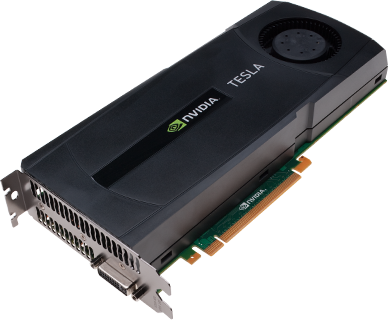
\includegraphics[width=0.2\textwidth]{tesla.png}\quad
        }
        \uncover<1,2,4>{
            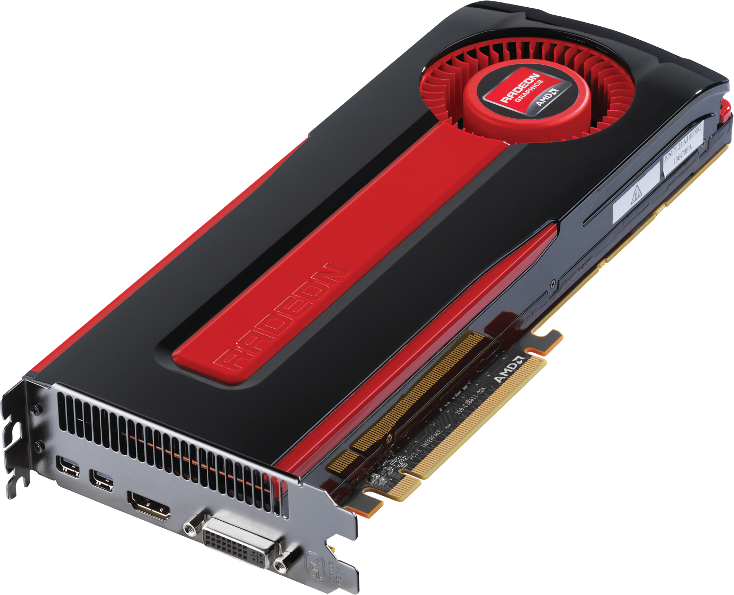
\includegraphics[width=0.2\textwidth]{radeon.png}\quad
        }
        \uncover<1,3>{
            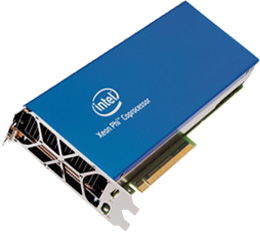
\includegraphics[width=0.17\textwidth]{intel.png}
        }
    \end{figure}
\end{frame}

\note[itemize]{
\item VexCL can transparently work with several compute devices that are
    present on your system.
\item We initialize the VexCL context with a device filter. The device filter
    is a simple functor that acts on cl::Device reference and returns a boolean
    value. Several standard filters are provided and you can write your own
    filters.
\item Let's assume that we have an NVIDIA GPU, an AMD GPU, and an Intel CPU
    installed.
    \begin{enumerate}
        \item The standard 'All' Filter select any device available, so we end
            with three devices in our context.
        \item If we want to select only GPUs, then we can filter the devices by
            type.
        \item It is also possible to combine the device filters with logical
            operators.  Here we select a GPU that is provided by AMD OpenCL
            platform.
        \item And here is an example of a custom filter. Here it selects any
            device that has at least 4GB of memory.
    \end{enumerate}
}

\subsection{Memory and work splitting}

%----------------------------------------------------------------------------
\begin{frame}[fragile]{Memory and work splitting}
    \setbeamercovered{transparent=40}
    \begin{exampleblock}{}
        \begin{onlyenv}<1|handout:0>
        \begin{lstlisting}
vex::Context ctx( vex::Filter::Name("Tesla") );
        \end{lstlisting}
        \end{onlyenv}
        \begin{onlyenv}<2|handout:0>
        \begin{lstlisting}
vex::Context ctx( vex::Filter::Type(CL_DEVICE_TYPE_GPU) );
        \end{lstlisting}
        \end{onlyenv}
        \begin{onlyenv}<3>
        \begin{lstlisting}
vex::Context ctx( vex::Filter::DoublePrecision );
        \end{lstlisting}
        \end{onlyenv}
        \begin{uncoverenv}<1>
        \begin{lstlisting}[firstnumber=last]

vex::vector<double> x(ctx, N);
vex::vector<double> y(ctx, N);

x = vex::element_index() * (1.0 / N);
y = sin(2 * x) + sqrt(1 - x * x);
        \end{lstlisting}
        \end{uncoverenv}
    \end{exampleblock}
    \setbeamercovered{invisible}
    \begin{figure}
        \begin{tikzpicture}
            \draw (0,2.5) rectangle +(8,0.1);
            \draw (0,2.5) grid[step=0.1] +(8,0.1);
            \draw (-0.3,2.6) node{x};

            \draw (0,2.0) rectangle +(8,0.1);
            \draw (0,2.0) grid[step=0.1] +(8,0.1);
            \draw (-0.3,2.1) node[anchor=center]{y};

            \uncover<1-3> {
            \draw (1,0.5) node{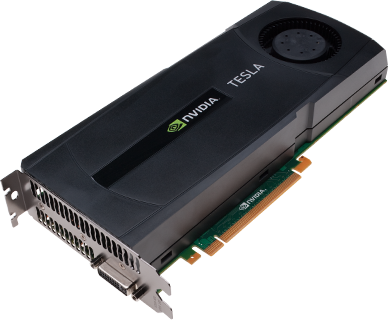
\includegraphics[width=0.2\textwidth]{tesla.png}};
            }

            \uncover<2-3> {
            \draw (4,0.5) node{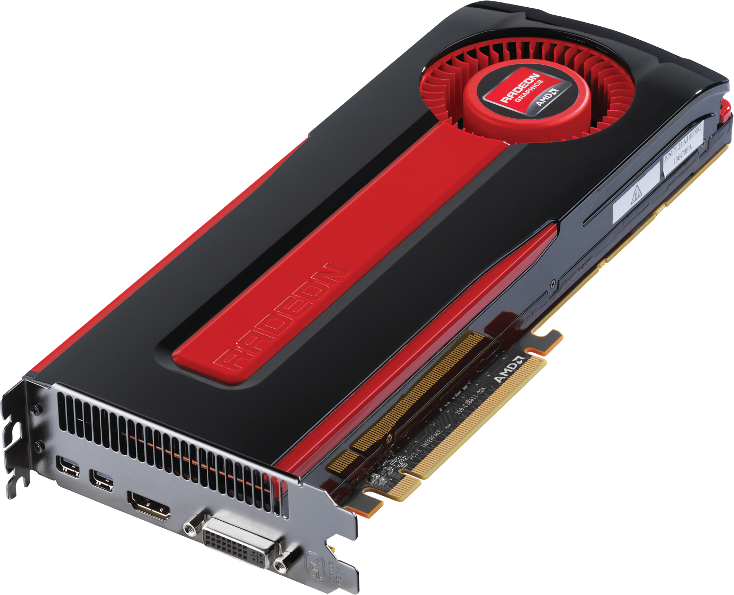
\includegraphics[width=0.2\textwidth]{radeon.png}};
            }

            \uncover<3> {
            \draw (7.5,0.5) node{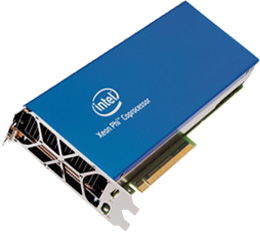
\includegraphics[width=0.17\textwidth]{intel.png}};
            }

            \uncover<1|handout:0> {
            \draw[->,chameleon3,style=dashed] (0,2.7) -- (0,1.8)
                .. controls +(east:0.5) and +(north west:0.5) ..
                (1.4,1.5);
            \draw[->,chameleon3,style=dashed] (8,2.7) -- (8,1.8)
                .. controls +(west:0.5) and +(north east:0.5) ..
                (1.6,1.5);
            }

            \uncover<2|handout:0> {
            \draw[->,chameleon3,style=dashed] (0,2.7) -- (0,1.8)
                .. controls +(east:0.5) and +(north west:0.5) ..
                (1.4,1.5);
            \draw[->,chameleon3,style=dashed] (4,2.7) -- (4,1.8)
                .. controls +(west:0.5) and +(north east:0.5) ..
                (1.6,1.5);

            \draw[->,chameleon3,style=dashed] (4,2.7) -- (4,1.8)
                .. controls +(east:0.1) and +(north west:0.2) ..
                (4.4,1.5);
            \draw[->,chameleon3,style=dashed] (8,2.7) -- (8,1.8)
                .. controls +(west:0.5) and +(north east:0.5) ..
                (4.6,1.5);
            }

            \uncover<3> {
            \draw[->,chameleon3,style=dashed] (0,2.7) -- (0,1.8)
                .. controls +(east:0.5) and +(north west:0.5) ..
                (1.4,1.5);
            \draw[->,chameleon3,style=dashed] (3,2.7) -- (3,1.8)
                .. controls +(west:0.5) and +(north east:0.5) ..
                (1.6,1.5);

            \draw[->,chameleon3,style=dashed] (3,2.7) -- (3,1.8)
                .. controls +(east:0.5) and +(north west:0.2) ..
                (4.4,1.5);
            \draw[->,chameleon3,style=dashed] (6,2.7) -- (6,1.8)
                .. controls +(west:0.5) and +(north east:0.5) ..
                (4.6,1.5);

            \draw[->,chameleon3,style=dashed] (6,2.7) -- (6,1.8) -- (7.4,1.5);
            \draw[->,chameleon3,style=dashed] (8,2.7) -- (8,1.8) -- (7.6,1.5);
            }
        \end{tikzpicture}
    \end{figure}
\end{frame}

\note[itemize]{
\item Now that we know how to initialize VexCL context, let's see how device
    vectors are allocated.
\item Here we allocate three vectors, and initialize two of them with
    constant values.
\item Each vector receives a list of queues at initialization.  Since each
    queue corresponds to a specific device, vectors know where to put their
    data to.
    \begin{enumerate}
        \item For example, if we only have the Tesla card in our context, then
            it will hold the complete memory for all of our vectors.
        \item If we use both of the available GPUs, then the vectors will be
            split between the devices. This split is by default proportional to
            the GPU bandwidth and is guaranteed to be consistent for vectors of
            the same size. This consistency allows VexCL to run computations
            independently on all devices in context.
        \item If we add the CPU to the context, it will get smaller share of
            the data and arithmetic operations.
    \end{enumerate}
\item Care must be taken with the use of several devices. VexCL tries to split
    the memory as fair as it can, but it is probable that your program will
    run at the speed of the slowest device.
}

\subsection{Supported expressions}
%----------------------------------------------------------------------------
\begin{frame}[fragile]{What vector expressions are supported?}
    \begin{itemize}
        \item All vectors in an expression have to be \emph{compatible}:
            \begin{itemize}
                \item Have same size
                \item Located on same devices
            \end{itemize}
        \item What may be used:
            \begin{columns}
                \begin{column}{0.4\textwidth}
                    \begin{itemize}
                        \item Vectors, scalars, constants
                        \item Arithmetic, logical operators
                        \item Built-in functions
                        \item User-defined functions
                        \item Random number generators
                        \item Slicing and permutations
                    \end{itemize}
                \end{column}
                \begin{column}{0.42\textwidth}
                    \begin{itemize}
                        \item Reduce to a scalar (sum, min, max)
                        \item Reduce across chosen dimensions
                        \item Stencil operations
                        \item Sparse matrix~-- vector products
                        \item Fast Fourier Transform
                        \item Sort, scan, reduce by key
                    \end{itemize}
                \end{column}
            \end{columns}
    \end{itemize}
\end{frame}

\note[itemize]{
\item So, what kind of expressions can you use in VexCL?
\item First, any vectors used in an expression have to be compatible.
\item If this requirement is satisfied, then expressions may combine
    vectors and scalars with almost any binary operators. OpenCL math functions
    and user-defined functions are also available.
}

%----------------------------------------------------------------------------
\begin{frame}[fragile]{A more involved example: Monte Carlo $\pi$}
    \begin{columns}
        \begin{column}{0.55\textwidth}
            \begin{itemize}
                \item Compute approximate value of $\pi$:
            \end{itemize}
            \vspace{\baselineskip}
            \begin{equation*}
                \frac{\text{area of circle}}{\text{area of square}} =
                \frac{\pi r^2}{(2r)^2} = \frac{\pi}{4},
            \end{equation*}
            \begin{equation*}
                \pi = 4 \frac{\text{area of circle}}{\text{area of square}}
                \approx 4 \frac{\text{\color{chameleon3}{points in
                circle}}}{\text{\color{chameleon3}{all}
                \color{chameleon1}{points}}}
            \end{equation*}
        \end{column}
        \begin{column}{0.35\textwidth}
            \begin{figure}
                \includegraphics[width=\textwidth]{mcpi}
            \end{figure}
        \end{column}
    \end{columns}
    \begin{exampleblock}{}
        \begin{lstlisting}
vex::Random<cl_double2> rnd;
vex::Reductor<size_t, vex::SUM> sum(ctx);

double pi = 4.0 * sum( length( rnd(vex::element_index(0, n), seed) ) < 1 ) / n;
        \end{lstlisting}
    \end{exampleblock}
\end{frame}

\note[itemize]{
\item Here is a bit more complex example of what you can do with VexCL.
\item Imagine we want to compute an approximate value of $\pi$ with Monte-Carlo
    method. We can use the following equalities to do this.
}

%----------------------------------------------------------------------------
\begin{frame}[fragile]{OpenCL/CUDA code is generated at runtime}
    \begin{columns}
        \begin{column}{0.38\textwidth}
            \begin{exampleblock}{This expression:}
                \begin{lstlisting}
x = 2 * y - sin(z);
                \end{lstlisting}
            \end{exampleblock}
        \end{column}
        \begin{column}{0.55\textwidth}
            \begin{exampleblock}{when compiled with:}
                \begin{onlyenv}<1>
                    \begin{lstlisting}[language=bash,numbers=none]
g++ -DVEXCL_BACKEND_OPENCL -lOpenCL ...
                    \end{lstlisting}
                \end{onlyenv}
                \begin{onlyenv}<2|handout:0>
                    \begin{lstlisting}[language=bash,numbers=none]
g++ -DVEXCL_BACKEND_CUDA -lcuda ...
                    \end{lstlisting}
                \end{onlyenv}
            \end{exampleblock}
        \end{column}
    \end{columns}
    \begin{exampleblock}{generates, compiles, and launches the following kernel
        at runtime:}
        \begin{onlyenv}<1>
            \begin{lstlisting}
kernel void vexcl_vector_kernel
(
  ulong n,
  global double * prm_1,        // x
  int prm_2,                    // 2
  global double * prm_3,        // y
  global double * prm_4         // z
)
{
  for(ulong idx = get_global_id(0); idx < n; idx += get_global_size(0))
  {
    prm_1[idx] = ( ( prm_2 * prm_3[idx] ) - sin( prm_4[idx] ) );
  }
}
            \end{lstlisting}
        \end{onlyenv}
        \begin{onlyenv}<2|handout:0>
            \begin{lstlisting}
extern "C" __global__ void vexcl_vector_kernel (
  ulong n,
  double * prm_1,               // x
  int prm_2,                    // 2
  double * prm_3,               // y
  double * prm_4                // z
)
{
  for(ulong idx = blockDim.x * blockIdx.x + threadIdx.x, grid_size = blockDim.x * gridDim.x;
      idx < n; idx += grid_size)
  {
    prm_1[idx] = ( ( prm_2 * prm_3[idx] ) - sin( prm_4[idx] ) );
  }
}
            \end{lstlisting}
        \end{onlyenv}
    \end{exampleblock}
\end{frame}

\note{ }

%----------------------------------------------------------------------------
\begin{frame}
    \begin{center}
        \huge{How does it work?}
    \end{center}
\end{frame}

\note{ }

%----------------------------------------------------------------------------
\section{Expression templates}
\begin{frame}
    \sectionpage
\end{frame}

\note{}

%----------------------------------------------------------------------------
\begin{frame}{Expression templates}
    \begin{itemize}
        \item How to implement a DSL in \CXX \emph{effectively}?
            \vspace{\baselineskip}
        \item The idea is quite old:
            \begin{description}[1995:]
                \item[1995:] \emph{Todd Veldhuizen}, Expression templates,
                    \CXX Report.
                \item[1996:]
                    Blitz{\raisebox{.2ex}{\relsize{-3}\bf ++}}\xspace is a \CXX
                    class library for scientific computing\\
                    \emph{which provides performance on par with Fortran
                    77/90}.
            \end{description}
        \item Today:
            \begin{itemize}
                \item Armadillo, Blaze, Boost.uBLAS, Eigen, MTL, etc.
            \end{itemize}
            \vspace{\baselineskip}
        \item \alert{\emph{But how does it work?}}
    \end{itemize}
\end{frame}

\note{ }

%----------------------------------------------------------------------------
\begin{frame}[fragile]{Simple example: Vector arithmetic}
    \begin{exampleblock}{We want to be able to write:}
        \begin{lstlisting}
x = y + z;
        \end{lstlisting}
    \end{exampleblock}

    \begin{exampleblock}{and it has to be as effective as:}
        \begin{lstlisting}
for(size_t i = 0; i < n; ++i)
    x[i] = y[i] + z[i];
        \end{lstlisting}
    \end{exampleblock}
\end{frame}

\note{ }

%----------------------------------------------------------------------------
\begin{frame}[fragile]{\CXX allows us to overload operators!}
    \begin{exampleblock}{}
        \begin{lstlisting}
vector operator+(const vector &a, const vector &b) {
    vector tmp( a.size() );
    for(size_t i = 0; i < a.size(); ++i)
        tmp[i] = a[i] + b[i];
    return tmp;
}
        \end{lstlisting}
    \end{exampleblock}
    \begin{itemize}
        \item Any problems?
            \begin{itemize}
                \item<2> Extra memory allocation
                \item<2> Extra memory I/O
            \end{itemize}
    \end{itemize}
    \begin{uncoverenv}<2>
        \begin{columns}
            \begin{column}{0.45\textwidth}
                \begin{exampleblock}{}
                    \begin{lstlisting}[aboveskip=0.4\baselineskip,belowskip=0.4\baselineskip]
a = x + y + z;

                    \end{lstlisting}
                \end{exampleblock}
                \begin{itemize}
                    \item 2 temporary vectors
                    \item $8 \times \text{n}$ memory reads/writes
                \end{itemize}
            \end{column}
            \begin{column}{0.45\textwidth}
                \begin{exampleblock}{}
                    \begin{lstlisting}
for(size_t i = 0; i < n; ++i)
    a[i] = x[i] + y[i] + z[i];
                    \end{lstlisting}
                \end{exampleblock}
                \begin{itemize}
                    \item no temporaries
                    \item $4 \times \text{n}$ memory reads/writes
                \end{itemize}
            \end{column}
        \end{columns}
    \end{uncoverenv}
\end{frame}

\note{
    Sometimes obvious solutions are the right ones\ldots
}

%----------------------------------------------------------------------------
\begin{frame}[fragile]{Lazy evaluation v0.1}
    \begin{description}
        \item[The idea:] postpone the actual evaluation until assignment.
    \end{description}
    \pause
    \begin{exampleblock}{}
        \begin{lstlisting}
struct vsum {
    const vector &lhs;
    const vector &rhs;
};
        \end{lstlisting}
        \pause
        \begin{lstlisting}[firstnumber=last]

vsum operator+(const vector &a, const vector &b) {
    return vsum{a, b};
}
        \end{lstlisting}
        \pause
        \begin{lstlisting}[firstnumber=last]

const vector& vector::operator=(const vsum &s) {
    for(size_t i = 0; i < n; ++i)
        data[i] = s.lhs[i] + s.rhs[i];
    return *this;
}
        \end{lstlisting}
    \end{exampleblock}
\end{frame}

\note{ }

%----------------------------------------------------------------------------
\begin{frame}[fragile]{Problem: its not composable}
    \begin{exampleblock}{What will happen here?}
        \begin{lstlisting}
a = x + y + z;
        \end{lstlisting}
    \end{exampleblock}

    \begin{exampleblock}<2>{}
        \begin{verbatim}
lazy_v1.cpp:38:15: error: invalid operands to binary expression
      ('vsum' and 'vector')
    a = x + y + z;
        ~~~~~ ^ ~
lazy_v1.cpp:12:12: note: candidate function not viable:
      no known conversion from 'vsum' to 'const vector' for 1st argument
vsum operator+(const vector &a, const vector &b) {
     ^
1 error generated.
        \end{verbatim}
    \end{exampleblock}
\end{frame}

\note{ }

%----------------------------------------------------------------------------
\begin{frame}[fragile,shrink=2]{Lazy evaluation v0.2}
    \begin{exampleblock}{}
        \begin{lstlisting}
template <class LHS, class RHS>
struct vsum {
    const LHS &lhs;
    const RHS &rhs;

    double operator[ ](size_t i) const { return lhs[i] + rhs[i]; }
};
        \end{lstlisting}
        \pause
        \begin{lstlisting}[firstnumber=last]

template <class LHS, class RHS>
vsum<LHS, RHS> operator+(const LHS &a, const RHS &b) {
    return vsum<LHS, RHS>{a, b};
}
        \end{lstlisting}
        \pause
        \begin{lstlisting}[firstnumber=last]

template<class Expr>
const vector& vector::operator=(const Expr &expr) {
    for(int i = 0; i < n; ++i) data[i] = expr[i];
    return *this;
}
        \end{lstlisting}
    \end{exampleblock}
\end{frame}

\note{ }

%----------------------------------------------------------------------------
\begin{frame}{Problem: its not general enough}
    \begin{figure}
        \begin{tikzpicture}
            \draw ( 0.0, 0.0) node{
\includegraphics[width=0.75\textwidth]{times_in_life}};
            \draw (-4.2,-3.4) node{\href{http://www.youtube.com/watch?v=j4o2PDwKdcA}{
\includegraphics[width=0.15\textwidth]{like}}};
            \draw ( 1.8, 0.8) node{There are times in life};
            \draw ( 1.8,-0.1) node{\Large when addition alone};
            \draw ( 1.8,-1.2) node{\Huge is not enough};
        \end{tikzpicture}
    \end{figure}
\end{frame}

\note{ }

%----------------------------------------------------------------------------
\begin{frame}[fragile]{Lazy evaluation v0.3}
    \begin{exampleblock}{}
        \begin{lstlisting}
struct plus {
    static double apply(double a, double b) { return a + b; }
};
        \end{lstlisting}
        \pause
        \begin{lstlisting}[firstnumber=last]

template <class LHS, class OP, class RHS>
struct binary_op {
    const LHS &lhs;
    const RHS &rhs;

    double operator[ ](size_t i) const { return OP::apply(lhs[i], rhs[i]); }
};
        \end{lstlisting}
        \pause
        \begin{lstlisting}[firstnumber=last]

template <class LHS, class RHS>
binary_op<LHS, plus, RHS> operator+(const LHS &a, const RHS &b) {
    return binary_op<LHS, plus, RHS>{a, b};
}
        \end{lstlisting}
    \end{exampleblock}
\end{frame}

\note{ }

%----------------------------------------------------------------------------
\begin{frame}[fragile]{Expression templates are trees}
    \begin{columns}
        \begin{column}{0.4\textwidth}
            \begin{exampleblock}{The expression in the RHS of:}
                \begin{onlyenv}<1>
                    \begin{lstlisting}
a = x + y;
                    \end{lstlisting}
                \end{onlyenv}
                \begin{onlyenv}<2->
                    \begin{lstlisting}
a = x + y - z;
                    \end{lstlisting}
                \end{onlyenv}
            \end{exampleblock}
            \begin{exampleblock}{... is of type:}
                \begin{uncoverenv}<2->
                    \begin{lstlisting}[numbers=none]
binary_op<
                    \end{lstlisting}
                \end{uncoverenv}
                \begin{lstlisting}[numbers=none]
    binary_op<
        vector,
        plus,
        vector
    >
                \end{lstlisting}
                \begin{uncoverenv}<2->
                    \begin{lstlisting}[numbers=none]
    , minus
    , vector
>
                    \end{lstlisting}
                \end{uncoverenv}
            \end{exampleblock}
        \end{column}
        \begin{column}{0.55\textwidth}
            \begin{figure}
                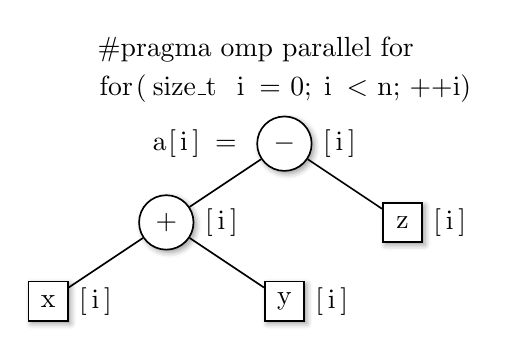
\begin{tikzpicture}
                    \uncover<2->{
                    \draw (0,0) node(sub)            [treenode,circle]{$-$};
                    \draw (sub) +( 1.50,-1) node(z)  [treenode,minimum size=0.5cm]{z};
                    }
                    \draw (sub) +(-1.50,-1) node(add)[treenode,circle]{$+$};
                    \draw (add) +(-1.50,-1) node(x)  [treenode,minimum size=0.5cm]{x};
                    \draw (add) +( 1.50,-1) node(y)  [treenode,minimum size=0.5cm]{y};

                    \uncover<2->{
                    \draw (sub) -- (add);
                    \draw (sub) -- (z);
                    }
                    \draw (add) -- (x);
                    \draw (add) -- (y);

                    \uncover<6->{
                        \draw (sub) +(-2.5, 1.2) node[anchor=west]{\code{#pragma omp parallel for}};
                    }
                    \uncover<3->{
                        \draw (sub) +(-2.5, 0.7) node[anchor=west]{\code{for(size_t i = 0; i < n; ++i)}};
                        \draw (sub) +(-1.8, 0.0) node[anchor=west]{\code{a[i] =}};
                    }
                    \uncover<3> {\draw (sub) +(0.7, 0) node{\code{[i]}};}
                    \uncover<4> {\draw (add) +(0.7, 0) node{\code{[i]}};}
                    \uncover<4->{\draw (z)   +(0.6, 0) node{\code{[i]}};}
                    \uncover<5->{\draw (x)   +(0.6, 0) node{\code{[i]}};}
                    \uncover<5->{\draw (y)   +(0.6, 0) node{\code{[i]}};}
                \end{tikzpicture}
            \end{figure}
            \begin{uncoverenv}<7>
                \begin{itemize}
                    \item The \CXX compiler walks the tree.
                    \item \code{binary_op::operator[ ]} does the actual work.
                \end{itemize}
            \end{uncoverenv}
        \end{column}
    \end{columns}
\end{frame}

\note{
}

%----------------------------------------------------------------------------
\begin{frame}[fragile]{So far, so good}
    \begin{exampleblock}{It is now possible to:}
        \begin{lstlisting}
v = a * x + b * y;

double c = (x + y)[42];
        \end{lstlisting}
    \end{exampleblock}

    \begin{exampleblock}{... and its as effective as:}
        \begin{lstlisting}
for(size_t i = 0; i < n; ++i)
    v[i] = a[i] * x[i] + b[i] * y[i];

double c = x[42] + y[42];
        \end{lstlisting}
    \end{exampleblock}
    \begin{itemize}
        \item No temporaries involved.
        \item Optimizing compiler is able to inline everything.
            \vspace{\baselineskip}
            \pause
        \item<alert@2> \emph{But how is that related to OpenCL code generation?}
    \end{itemize}
\end{frame}

\note{
    It turns out that once you understand how expression templates are working,
    it is really easy to shift to code generation.
}

%----------------------------------------------------------------------------
\section{OpenCL code generation}
\begin{frame}
    \sectionpage
\end{frame}

\note{ }

%----------------------------------------------------------------------------
\begin{frame}{How does OpenCL work?}
    \begin{enumerate}
        \item A compute kernel is compiled at runtime from \CC source.
        \item Kernel parameters are set through API calls.
        \item Kernel is launched on a compute device.
    \end{enumerate}
    \vspace{\baselineskip}
    \pause
    \begin{itemize}
        \item Source may be read from a file, or stored in a static
            string, or \alert{\emph{generated}}.
    \end{itemize}
\end{frame}

\note{ }

%----------------------------------------------------------------------------
\begin{frame}[fragile]{Generating kernel source from an expression}
    \begin{exampleblock}{We want this expression:}
        \begin{lstlisting}
a = x + y - z;
        \end{lstlisting}
    \end{exampleblock}
    \begin{exampleblock}{\ldots to result in this kernel:}
        \begin{lstlisting}
kernel void vexcl_vector_kernel(
    ulong n,
    global double * res,
    global double * prm1,
    global double * prm2,
    global double * prm3
)
{
    for(size_t idx = get_global_id(0); idx < n; idx += get_global_size(0)) {
        res[idx] = ( ( prm1[idx] + prm2[idx] ) - prm3[idx] );
    }
}
        \end{lstlisting}
    \end{exampleblock}
    \begin{tikzpicture}[overlay,scale=0.8]
        \draw (11,6) node(sub)[treenode,circle]{$-$};
        \draw (sub) +( 1.50,-1) node(z)  [treenode,minimum size=0.5cm]{z};
        \draw (sub) +(-1.50,-1) node(add)[treenode,circle]{$+$};
        \draw (add) +(-1.50,-1) node(x)  [treenode,minimum size=0.5cm]{x};
        \draw (add) +( 1.50,-1) node(y)  [treenode,minimum size=0.5cm]{y};
        \draw (sub) -- (add);
        \draw (sub) -- (z);
        \draw (add) -- (x);
        \draw (add) -- (y);
    \end{tikzpicture}
\end{frame}

\note{ }

%----------------------------------------------------------------------------
\begin{frame}[fragile]{Declaring parameters}
    \begin{exampleblock}{Each terminal knows what parameters it needs:}
        \begin{lstlisting}
/*static*/ void vector::declare_params(std::ostream &src, unsigned &pos) {
    src << ",\n    global double * prm" << ++pos;
}
        \end{lstlisting}
    \end{exampleblock}
    \begin{exampleblock}{An expression just asks its terminals to do the work:}
        \begin{lstlisting}[firstnumber=last]
template <class LHS, class OP, class RHS>
/*static*/ void binary_op<LHS, OP, RHS>::declare_params(
                            std::ostream &src, unsigned &pos)
{
    LHS::declare_params(src, pos);
    RHS::declare_params(src, pos);
}
        \end{lstlisting}
    \end{exampleblock}
\end{frame}

\note{ }

%----------------------------------------------------------------------------
\begin{frame}[fragile]{Building string representation for expression}
    \begin{exampleblock}{}
        \begin{lstlisting}
struct plus {
    static std::string to_string(std::ostream &src) { src << " + "; }
};
        \end{lstlisting}
        \pause
        \begin{lstlisting}[firstnumber=last]

/*static*/ void vector::to_string(std::ostream &src, unsigned &pos) {
    src << "prm" << ++pos << "[idx]";
}
        \end{lstlisting}
        \pause
        \begin{lstlisting}[firstnumber=last]

template <class LHS, class OP, class RHS>
/*static*/ void binary_op<LHS, OP, RHS>::to_string(std::ostream &src, unsigned &pos) {
    src << "( ";
    LHS::to_string(src, pos);
    OP::to_string(src);
    RHS::to_string(src, pos);
    src << " )";
}
        \end{lstlisting}
    \end{exampleblock}
\end{frame}

\note[itemize]{
\item The obvious observation is that\ldots
}

%----------------------------------------------------------------------------
\begin{frame}[fragile]{Generating kernel source}
    \setbeamercovered{transparent=40}
    \begin{exampleblock}{}
        \begin{uncoverenv}<1>
            \begin{lstlisting}
template <class LHS, class RHS>
std::string kernel_source() {
    std::ostringstream src;

    src << "kernel void vexcl_vector_kernel(\n    ulong n";
            \end{lstlisting}
        \end{uncoverenv}
        \begin{uncoverenv}<1,2>
            \begin{lstlisting}[firstnumber=last]
    unsigned pos = 0;
    LHS::declare_params(src, pos);
    RHS::declare_params(src, pos);
            \end{lstlisting}
        \end{uncoverenv}
        \begin{uncoverenv}<1>
            \begin{lstlisting}[firstnumber=last]
    src << ")\n{\n"
            "    for(size_t idx = get_global_id(0); idx < n; idx += get_global_size(0)) {\n"
            "        ";
            \end{lstlisting}
        \end{uncoverenv}
        \begin{uncoverenv}<1,3>
            \begin{lstlisting}[firstnumber=last]
    pos = 0;
    LHS::to_string(src, pos); src << " = ";
    RHS::to_string(src, pos); src << ";\n";
            \end{lstlisting}
        \end{uncoverenv}
        \begin{uncoverenv}<1>
            \begin{lstlisting}[firstnumber=last]
    src << "    }\n}\n";

    return src.str();
}
            \end{lstlisting}
        \end{uncoverenv}
    \end{exampleblock}
\end{frame}

\note{ }

%----------------------------------------------------------------------------
\begin{frame}[fragile]{Setting kernel arguments}
    \begin{exampleblock}{}
        \begin{lstlisting}
void vector::set_args(cl::Kernel &krn, unsigned &pos) {
    krn.setArg(pos++, buffer);
}

template <class LHS, class OP, class RHS>
void binary_op<LHS, OP, RHS>::set_args(cl::Kernel &krn, unsigned &pos) {
    lhs.set_args(krn, pos);
    rhs.set_args(krn, pos);
}
        \end{lstlisting}
    \end{exampleblock}

    \vspace{\baselineskip}

    \begin{itemize}
        \item The methods are not static anymore!
    \end{itemize}
\end{frame}

\note{ }

%----------------------------------------------------------------------------
\begin{frame}[fragile]{Gluing it all together}
    \setbeamercovered{transparent=40}
    \begin{exampleblock}{}
        \begin{uncoverenv}<1>
            \begin{lstlisting}
template <class Expr>
const vector& vector::operator=(const Expr &expr) {
            \end{lstlisting}
        \end{uncoverenv}
        \begin{uncoverenv}<1,2>
            \begin{lstlisting}[firstnumber=last]
    static cl::Kernel krn = build_kernel(device, kernel_source<This, Expr>());
            \end{lstlisting}
        \end{uncoverenv}
        \begin{uncoverenv}<1>
            \begin{lstlisting}[firstnumber=last]

    unsigned pos = 0;

    krn.setArg(pos++, size);     // n
    krn.setArg(pos++, buffer);   // result
    expr.set_args(krn, pos);     // other parameters

    queue.enqueueNDRangeKernel(krn, cl::NullRange, buffer.size(), cl::NullRange);

    return *this;
}
            \end{lstlisting}
        \end{uncoverenv}
    \end{exampleblock}
    \setbeamercovered{transparent=0}
    \begin{uncoverenv}<2>
        \begin{itemize}
            \item Kernel is generated and compiled once, applied many times:
                \begin{itemize}
                    \item Each kernel is uniquely identified by its expression
                        type.
                    \item Hence, we may use local static variable to cache the
                        kernel.
                \end{itemize}
        \end{itemize}
    \end{uncoverenv}
\end{frame}

\note{ }

%----------------------------------------------------------------------------
\begin{frame}[fragile]{What you saw is not what you get}
    \begin{tikzpicture}[remember picture,overlay]
        \node[anchor=north east,yshift=4pt,xshift=4pt] at (current page.north east) {
            
\includegraphics[width=3.6cm]{clippy}
        };
    \end{tikzpicture}
    \begin{itemize}
        \item The actual implementation is a bit more complicated:
            \begin{itemize}
                \item There are unary, binary, n-ary expressions.
                \item There are special terminals requiring either global or
                    local preambles.
                \item There are builtin and user-defined functions.
                \item \ldots
            \end{itemize}
        \item Boost.Proto is used to keep the code mess contained.
    \end{itemize}
\end{frame}

\note[itemize] {
\item You are welcome to look at the actual code for more details.
}

%----------------------------------------------------------------------------
\section{Boost.Proto}

\begin{frame}[fragile]{Boost.Proto}
    \setbeamercovered{transparent=40}
    \begin{description}[\quad]
        \item[Boost.Proto]  is a framework for building Embedded
            Domain-Specific Languages in \CXX. It provides tools for
            constructing, type-checking, transforming and executing expression
            templates.
    \end{description}
    \begin{columns}
        \begin{column}[t]{0.6\textwidth}
            \begin{exampleblock}{Hello Proto}
                \begin{lstlisting}
#include <iostream>
#include <boost/proto/proto.hpp>
namespace proto = boost::proto;

int main() {
    auto expr = proto::as_expr(6) * 7 - 2;
                \end{lstlisting}
                \begin{uncoverenv}<1>
                    \begin{lstlisting}[firstnumber=last]
    proto::display_expr( expr );
                    \end{lstlisting}
                \end{uncoverenv}
                \begin{uncoverenv}<2>
                    \begin{lstlisting}[firstnumber=last]

    proto::default_context ctx;
    std::cout << proto::eval( expr, ctx ) << std::endl;
                    \end{lstlisting}
                \end{uncoverenv}
                \begin{lstlisting}[firstnumber=last]
}
                \end{lstlisting}
            \end{exampleblock}
        \end{column}
        \begin{column}[t]{0.35\textwidth}
            \begin{exampleblock}{Output:}
                \vspace{0.8\baselineskip}
                \begin{uncoverenv}<1>
                \begin{verbatim}
minus(
    multiplies(
        terminal(6)
      , terminal(7)
    )
  , terminal(2)
)
                \end{verbatim}
                \end{uncoverenv}
                \begin{uncoverenv}<2>
                \begin{verbatim}
40
                \end{verbatim}
                \end{uncoverenv}
                \vspace{0.9\baselineskip}
            \end{exampleblock}
        \end{column}
    \end{columns}
\end{frame}

\note[itemize]{
\item \code{proto::as_expr} is used to infect the expression, and brings
    Proto's tree-building operator overloads into consideration.
}

%----------------------------------------------------------------------------
\begin{frame}[fragile,shrink=5]{Creating custom Boost.Proto context}
    \begin{exampleblock}{1. Define custom Proto context:}
        \begin{lstlisting}
struct print_expression_context {
    template <typename Expr, typename Tag = typename Expr::proto_tag> struct eval {};

    template <typename Expr>
    struct eval<Expr, proto::tag::plus> {
        typedef void result_type;
        void operator()(const Expr &expr, print_expression_context &ctx) const {
            cout << "( ";
            proto::eval( proto::left (expr), ctx );
            cout << " + ";
            proto::eval( proto::right(expr), ctx );
            cout << " )";
        }
    };

    template <typename Expr>
    struct eval<Expr, proto::tag::terminal> {
        typedef void result_type;
        void operator()(const Expr &expr, print_expression_context &ctx) const {
            cout << proto::eval( expr, proto::default_context() );
        }
    };
};
        \end{lstlisting}
    \end{exampleblock}
\end{frame}

\note{}

%----------------------------------------------------------------------------
\begin{frame}[fragile]{Creating custom Boost.Proto context}
    \begin{exampleblock}{2. Use the context:}
        \begin{lstlisting}
auto expr = proto::as_expr(6) * 7 - 2;

print_expression_context ctx;
proto::eval( expr, ctx );
        \end{lstlisting}
    \end{exampleblock}

    \begin{exampleblock}{Output:}
        \begin{verbatim}
( ( 6 * 7 ) + 5 )
        \end{verbatim}
    \end{exampleblock}
\end{frame}

\note{}

%----------------------------------------------------------------------------
\begin{frame}[fragile]{Generating code with Boost.Proto}
    \setbeamercovered{transparent=40}
    \begin{exampleblock}{}
        \begin{lstlisting}
template <class Term> struct partial_vector_expr {
  static void get(std::ostream &os, unsigned &pos) { os << "prm_" << ++pos; }
};
        \end{lstlisting}
        \begin{uncoverenv}<2->
            \begin{lstlisting}[firstnumber=last]

struct print_expression_context {
  // ...
  unsigned pos = 0;

  template <typename Expr>
  struct eval<Expr, proto::tag::terminal> {
    typedef void result_type;
    void operator()(const Expr &expr, print_expression_context &ctx) const {
      partial_vector_expr<typename proto::result_of::value<Expr>::type>::get(cout, ctx.pos);
    }
  };
};
            \end{lstlisting}
        \end{uncoverenv}
    \end{exampleblock}
    \setbeamercovered{transparent=0}
    \begin{uncoverenv}<3>
        \begin{columns}
            \begin{column}{0.53\textwidth}
                \begin{exampleblock}{}
                    \begin{lstlisting}
proto::eval( proto::as_expr(6) * 7 - 2, ctx);
                    \end{lstlisting}
                \end{exampleblock}
            \end{column}
            \begin{column}{0.4\textwidth}
                \begin{exampleblock}{}
                    \begin{verbatim}
( ( prm_1 * prm_2 ) + prm_3 )
                    \end{verbatim}
                \end{exampleblock}
            \end{column}
        \end{columns}
    \end{uncoverenv}
\end{frame}

\note{}

%----------------------------------------------------------------------------
\begin{frame}{Almost there\ldots}
    \begin{itemize}
        \item The code is very close to the one actually used in VexCL
            \begin{itemize}
                \item We can leave definition of
                    \code{print_expression_context} intact.
                \item Only \code{partial_vector_expr} needs to be specialized
                    for each new terminal type.
            \end{itemize}
        \item We will need several contexts similar to
            \code{print_expression_context}:
            \begin{itemize}
                \item Declaring kernel parameters,
                \item Setting kernel arguments,
                \item \ldots
            \end{itemize}
    \end{itemize}
\end{frame}

\note{}

\section{Example: element index}
%----------------------------------------------------------------------------
\begin{frame}[fragile,shrink=10]{General structure of OpenCL code}
    \setbeamercovered{transparent=40}
    \begin{columns}
        \begin{column}{0.55\textwidth}
            \vspace{-0.5\baselineskip}
            \begin{exampleblock}{VexCL code:}
                    \begin{lstlisting}
VEX_FUNCTION(double, sqr, (double, x)(double, y),
        return x * x + y * y;
        );
auto tmp = vex::make_temp<1>(x);
y = sqr(sin(tmp), cos(tmp));
                    \end{lstlisting}
            \end{exampleblock}
            \begin{exampleblock}{OpenCL code:}
                \begin{uncoverenv}<1,2,6>
                    \begin{lstlisting}
double sqr(double x, double y) { return x * x + y * y; }
                    \end{lstlisting}
                \end{uncoverenv}
                \begin{uncoverenv}<1,6>
                    \begin{lstlisting}[firstnumber=last]
kernel void vexcl_vector_kernel (ulong n,
            \end{lstlisting}
        \end{uncoverenv}
        \begin{uncoverenv}<1,3,6>
            \begin{lstlisting}[firstnumber=last]
  global double * prm_1,
  global double * prm_2_1
            \end{lstlisting}
        \end{uncoverenv}
        \begin{uncoverenv}<1,6>
            \begin{lstlisting}[firstnumber=last]
)
{
  for(ulong idx = get_global_id(0);
      idx < n; idx += get_global_size(0))
  {
                    \end{lstlisting}
                \end{uncoverenv}
                \begin{uncoverenv}<1,4,6>
                    \begin{lstlisting}[firstnumber=last]
    double temp_1 = prm_2_1[idx];
                    \end{lstlisting}
                \end{uncoverenv}
                \begin{uncoverenv}<1,5,6>
                    \begin{lstlisting}[firstnumber=last]
    prm_1[idx] = sqr( sin( temp_1 ), cos( temp_1 ) );
                    \end{lstlisting}
                \end{uncoverenv}
                \begin{uncoverenv}<1,6>
                    \begin{lstlisting}[firstnumber=last]
  }
}
                    \end{lstlisting}
                \end{uncoverenv}
            \end{exampleblock}
        \end{column}
        \setbeamercovered{transparent=0}
        \begin{column}{0.38\textwidth}
            \begin{itemize}
                \item Each terminal should tell VexCL how to use it:
                    \begin{itemize}
                        \item<alert@2> Does the terminal need global preamble?
                        \item<alert@3> What kernel parameters does it need, and
                            how to set them?
                        \item<alert@4> Does it need local preamble?
                        \item<alert@5> What contribution does it make to
                            the expression string?
                    \end{itemize}
                    \vspace{\baselineskip}
                \item<6> This is done by specializing a number of templated
                    structs.
            \end{itemize}
        \end{column}
    \end{columns}
\end{frame}

\note{ }

%----------------------------------------------------------------------------
\begin{frame}[fragile]{Example: element index}{\code{<vexcl/element_index.hpp>}}
    \setbeamercovered{transparent=40}
    \begin{exampleblock}{}
        \begin{lstlisting}
x = sin( 2 * M_PI * vex::element_index() / n );
        \end{lstlisting}
    \end{exampleblock}
    \begin{exampleblock}{}
        \begin{onlyenv}<1-4>
            \begin{uncoverenv}<1-3>
                \begin{lstlisting}
namespace vex {
    struct elem_index {
        size_t offset;
    };
                \end{lstlisting}
            \end{uncoverenv}
            \begin{uncoverenv}<2-4>
                \begin{lstlisting}[firstnumber=last]

    inline auto element_index(size_t offset = 0) {
        return boost::proto::as_expr<vector_domain>( elem_index{offset} );
    }
                \end{lstlisting}
            \end{uncoverenv}
            \begin{uncoverenv}<3>
                \begin{lstlisting}[firstnumber=last]

    namespace traits {
        template <> struct is_vector_expr_terminal< elem_index > : std::true_type {};
    }
            \end{lstlisting}
        \end{uncoverenv}
        \begin{lstlisting}[firstnumber=last]
}
        \end{lstlisting}
        \end{onlyenv}
        \begin{onlyenv}<5->
        \begin{uncoverenv}<1>
            \begin{lstlisting}
namespace vex {
    struct elem_index {
        size_t offset;
    };
            \end{lstlisting}
        \end{uncoverenv}
        \begin{uncoverenv}<5>
            \begin{lstlisting}[firstnumber=last]

    inline boost::proto::result_of::as_expr<elem_index, vector_domain>::type
    element_index(size_t offset = 0) {
        return boost::proto::as_expr<vector_domain>( elem_index{offset} );
    }
            \end{lstlisting}
        \end{uncoverenv}
        \begin{uncoverenv}<1>
            \begin{lstlisting}[firstnumber=last]

    namespace traits {
        template <> struct is_vector_expr_terminal< elem_index > : std::true_type {};
    }
}
            \end{lstlisting}
        \end{uncoverenv}
        \end{onlyenv}
    \end{exampleblock}
\end{frame}

\note{ }

%----------------------------------------------------------------------------
\begin{frame}[fragile]{Parameter declaration}
    \setbeamercovered{transparent=40}
    \begin{exampleblock}{}
        \begin{lstlisting}
template <>
struct kernel_param_declaration< elem_index >
{
    static std::string get(
        const elem_index&, const cl::Device&, const std::string &prm_name,
        detail::kernel_generator_state_ptr
        )
    {
        std::ostringstream s;
        s << ",\n\t" << type_name<size_t>() << " " << prm_name;
        return s.str();
    }
};
        \end{lstlisting}
    \end{exampleblock}
\end{frame}

\note{ }

%----------------------------------------------------------------------------
\begin{frame}[fragile]{Contribution to expression string}
    \begin{exampleblock}{}
            \begin{lstlisting}
template <>
struct partial_vector_expr< elem_index >
{
    \end{lstlisting}
    \begin{lstlisting}[firstnumber=last]
    static std::string get(
        const elem_index&, const cl::Device&, const std::string &prm_name,
        detail::kernel_generator_state_ptr
        )
    \end{lstlisting}
    \begin{lstlisting}[firstnumber=last]
    {
        std::ostringstream s;
        s << "(" << prm_name << " + idx)";
        return s.str();
    }
    \end{lstlisting}
    \begin{lstlisting}[firstnumber=last]
};
            \end{lstlisting}
    \end{exampleblock}
\end{frame}

\note{ }

%----------------------------------------------------------------------------
\begin{frame}[fragile]{Setting kernel arguments}
    \begin{exampleblock}{}
        \begin{lstlisting}
template <>
struct kernel_arg_setter< elem_index >
{
    static void set(
        const elem_index &term, cl::Kernel &kernel, unsigned /*device*/,
        size_t index_offset, unsigned &position,
        detail::kernel_generator_state_ptr
        )
    {
        kernel.setArg(position++, term.offset + index_offset);
    }
};
        \end{lstlisting}
    \end{exampleblock}
\end{frame}

\note{ }

%----------------------------------------------------------------------------
\begin{frame}[fragile]{And we are done!}
    \begin{itemize}
        \item \code{vex::element_index()} is now fully defined:
            \begin{itemize}
                \item We may use it in vector expressions of arbitrary
                    complexity.
            \end{itemize}
            \vspace{\baselineskip}
        \item Also, we have an expression engine (a set of proto contexts):
            \begin{itemize}
                \item Adding new terminal types is straightforward.
            \end{itemize}
    \end{itemize}
\end{frame}

\note{}

%----------------------------------------------------------------------------
\section{Other uses for expression templates in VexCL}
\begin{frame}
    \sectionpage
\end{frame}

\note{}

%----------------------------------------------------------------------------
\begin{frame}[fragile]{Device filters}
    \begin{exampleblock}{}
        \begin{lstlisting}
vex::Context ctx(
                 vex::Filter::Env && vex::Filter::DoublePrecision
                );
        \end{lstlisting}
    \end{exampleblock}
    \begin{itemize}
        \item Mini-DSL inside VexCL
            \begin{itemize}
                \item Terminals are functors
                \item Only logical operators are provided
            \end{itemize}
    \end{itemize}
\end{frame}

\note{}

%----------------------------------------------------------------------------
\begin{frame}[fragile]{Symbolic variables}
    \begin{itemize}
        \item An instance of \code{vex::symbolic<>} dumps any arithmetic
            operations to a \code{std::ostream}:
            \vspace{-0.5\baselineskip}
    \end{itemize}
    \begin{columns}
        \begin{column}{0.45\textwidth}
            \begin{exampleblock}{}
                \begin{lstlisting}
vex::generator::set_recorder( std::cout );
vex::symbolic<double> x, y = 6;
x = sin(y * 7);
                \end{lstlisting}
            \end{exampleblock}
        \end{column}
        \begin{column}{0.45\textwidth}
            \begin{exampleblock}{}
                \begin{verbatim}
double var1;
double var2 = 6;
var1 = sin( var2 * 7 );
                \end{verbatim}
            \end{exampleblock}
        \end{column}
    \end{columns}
    \vspace{\baselineskip}
    \begin{itemize}
        \item We may feed symbolic variables to a generic algorithm and obtain
            its string representation.
            \begin{itemize}
                \item Generate VexCL function:
            \end{itemize}
    \begin{exampleblock}{}
        \begin{lstlisting}
auto sqr = vex::generator::make_function<double(double, double)>(
                [ ](const auto &x, const auto &y){ return x * x + y * y; } );
x = sqr( sin(y), cos(z) );
        \end{lstlisting}
    \end{exampleblock}
    \begin{itemize}
        \item Generate effective compute kernel from a generic algorithm.
    \end{itemize}
    \end{itemize}
\end{frame}

\note{}

%----------------------------------------------------------------------------
\section{Conclusion}
\begin{frame}[label=conclusion]{Conclusion}
    \begin{columns}
        \begin{column}{0.55\textwidth}
            \begin{itemize}
                \item Advantages of code generation:
                    \vspace{0.5\baselineskip}
                    \begin{itemize}
                        \item You get the exact kernel you need.
                            \vspace{0.5\baselineskip}
                        \item Flexibility of generic \CXX code\\
                            with \CC backend.
                            \vspace{0.5\baselineskip}
                        \item There is no need to use\\
                            vendor-specific solutions.
                            \vspace{\baselineskip}
                        \item Performance!
                    \end{itemize}
            \end{itemize}
        \end{column}
        \begin{column}{0.45\textwidth}
            \vspace{-1\baselineskip}
            \begin{figure}
                \begin{center}
                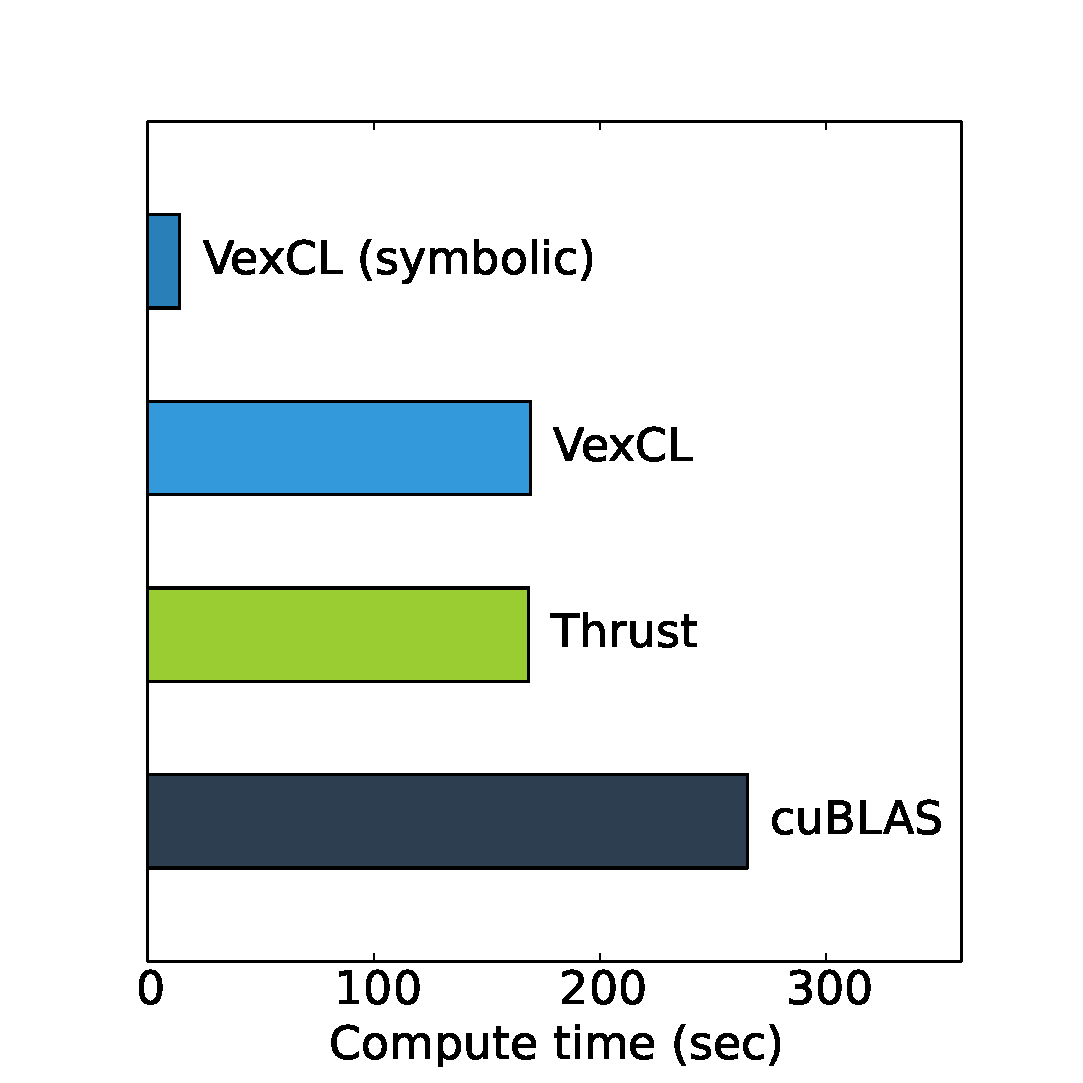
\includegraphics[width=\textwidth]{perfplot}

                \vspace{\baselineskip}
                {\small \sl
                    Integrate large number of ODEs\\
                    on a GPU with Boost.odeint
                }
            \end{center}
            \end{figure}
        \end{column}
    \end{columns}

    \forkme{east}{https://github.com/ddemidov/vexcl}%
\end{frame}

\note{}

%----------------------------------------------------------------------------
\appendix

%----------------------------------------------------------------------------
\section{Benchmarking performance}
\begin{frame}
    \sectionpage
\end{frame}

\note{}

%----------------------------------------------------------------------------
\begin{frame}[fragile]{Parameter study for the Lorenz attractor system}
    \begin{columns}
        \begin{column}{0.5\textwidth}
            \begin{block}{Lorenz attractor system}
                \vspace{-1\baselineskip}
                \begin{align*}
                    \dot{x} &= -\sigma \left( x - y \right), \\
                    \dot{y} &= R x - y - xz, \\
                    \dot{z} &= -bz + xy.
                    \label{eq:lorenz}
                \end{align*}
            \end{block}
            \begin{itemize}
                \item Solve large number of Lorenz systems, each
                    for a different value of $R$.
                \item Use Boost.odeint.
            \end{itemize}
        \end{column}
        \begin{column}{0.4\textwidth}
            \begin{figure}
                \begin{center}
                    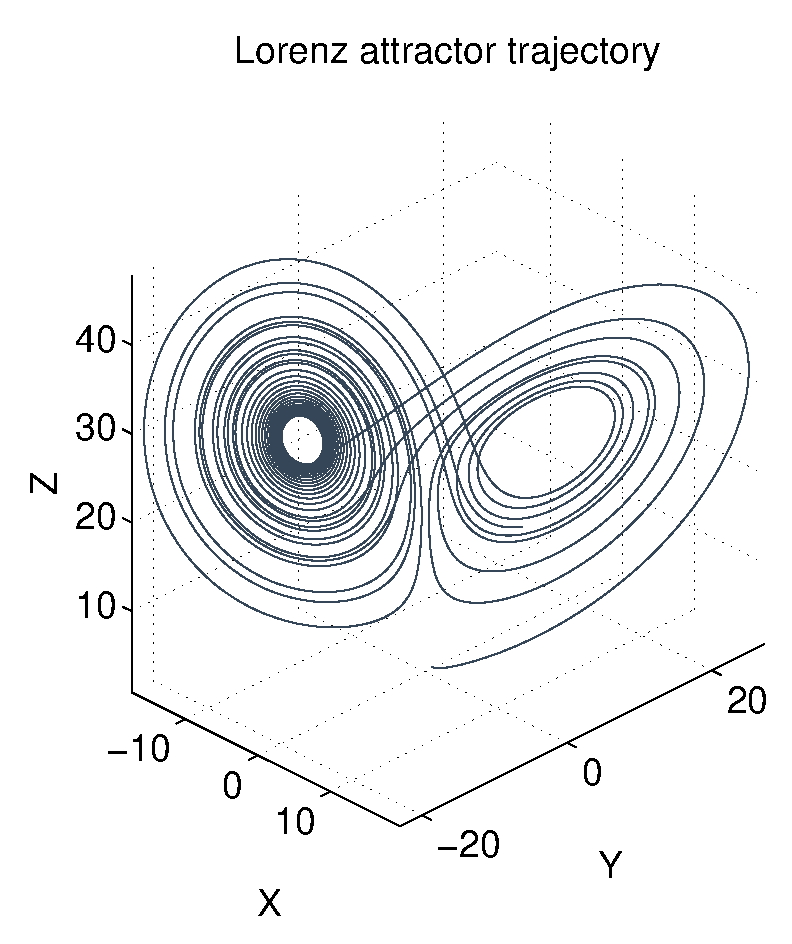
\includegraphics[width=\textwidth]{lorenz}

                    {\small \sl Lorenz attractor trajectory}
                \end{center}
            \end{figure}
        \end{column}
    \end{columns}
\end{frame}

\note[itemize]{
\item As an example, lets solve a Lorenz attractor system of ordinary
    differential equations.
\item Lorenz attractor is a particle that moves according to these governing
    equations. The plot on the right shows an example of particle trajectory in
    time.
\item We will solve large number of these Lorenz systems at once.  Each of the
    systems will have its own value for parameter R. That's why this is called
    a parameter study.
}

%----------------------------------------------------------------------------
\begin{frame}[fragile]{CUBLAS implementation}
    \begin{itemize}
        \item CUBLAS is a highly optimized BLAS implementation from NVIDIA.
        \item Its disadvantage is that it has fixed number of
            kernels/functions.
        \item Hence, linear combinations (used internally by odeint):
            \begin{equation*}
                x_0 = \alpha_1 x_1 + \alpha_2 x_2 + \cdots + \alpha_n x_n
            \end{equation*}
            are implemented as:
    \end{itemize}
    \begin{exampleblock}{}
        \begin{lstlisting}[numbers=none,texcl=true]
cublasDset(...);        // $x_0 = 0$
cublasDaxpy(...);       // $x_0 = x_0 + \alpha_1 * x_1$
...
cublasDaxpy(...);       // $x_0 = x_0 + \alpha_n * x_n$
        \end{lstlisting}
    \end{exampleblock}
\end{frame}

\note{ }

%----------------------------------------------------------------------------
\begin{frame}[fragile]{Thrust implementation}
    \begin{itemize}
        \item It is possible to fuse linear combination kernels with Thrust:
    \end{itemize}
    \begin{columns}
        \begin{column}{0.70\textwidth}
            \begin{exampleblock}{Thrust}
                \begin{adjustbox}{width=0.95\textwidth,height=0.6\textheight,keepaspectratio}
                    \begin{lstlisting}
struct scale_sum2 {
    const double a1, a2;
    scale_sum2(double a1, double a2) : a1(a1), a2(a2) { }
    template<class Tuple>
    __host__ __device__ void operator()(Tuple t) const {
        thrust::get<0>(t) = a1 * thrust::get<1>(t) + a2 * thrust::get<2>(t);
    }
};

thrust::for_each(
        thrust::make_zip_iterator(
            thrust::make_tuple( x0.begin(), x1.begin(), x2.begin() )
            ),
        thrust::make_zip_iterator(
            thrust::make_tuple( x0.end(), x1.end(), x2.end() )
            ),
        scale_sum2(a1, a2)
        );
                    \end{lstlisting}
                \end{adjustbox}
            \end{exampleblock}
        \end{column}
        \begin{column}<2>{0.22\textwidth}
            \begin{exampleblock}{VexCL}
                \begin{adjustbox}{width=0.95\textwidth,height=0.6\textheight,keepaspectratio}
                    \begin{lstlisting}
x0 = a1 * x1 + a2 * x2;
                    \end{lstlisting}
                \end{adjustbox}
            \end{exampleblock}
        \end{column}
    \end{columns}
\end{frame}

\note{ }

%----------------------------------------------------------------------------
\begin{frame}[fragile]{VexCL symbolic implementation}
    \begin{itemize}
        \item Pass VexCL symbolic variables to a Boost.odeint algorithm.
        \item Make single integration step.
        \item Generate monolithic kernel that does one full time step.
            \begin{itemize}
                \item Intermediate variables are no longer stored in global
                    memory.
            \end{itemize}
    \end{itemize}
\end{frame}

\note{ }

%----------------------------------------------------------------------------
\againframe{conclusion}

\end{document}
